\documentclass{standalone}
\usepackage{plots}
\usepackage{hyperref}

\def\rawrsversion{0.6.4}
\newcommand\doclink[1]{\underline{\texttt{#1}}}
\newcommand\rsdocs[2]{\href{https://docs.rs/rustsat/\rawrsversion/rustsat/#2}{\doclink{#1}}}
\newcommand\crate[1]{\href{https://crates.io/crates/#1}{\doclink{#1}}}
\newcommand\module[1]{\rsdocs{#1}{#1}}

\begin{document}
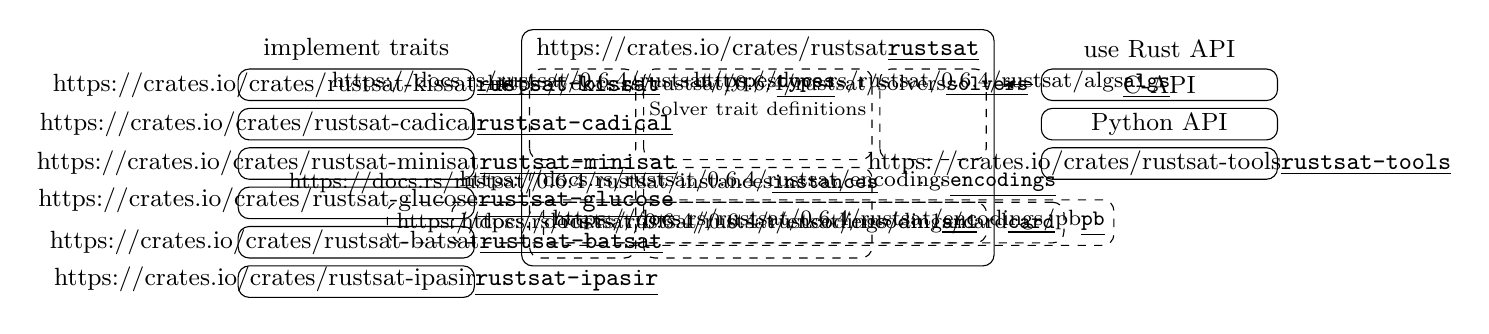
\begin{tikzpicture}[
  font=\small,
  crate/.style={rounded corners},
  mod/.style={rounded corners,dashed},
]
  \def\width{6}
  \def\height{3}

  \draw [crate] (0,0) rectangle (\width,\height);
  \node at (.5*\width,\height-.25) {\crate{rustsat}};

  \draw [mod] (.1,\height/2-.15) rectangle ++(\width/4-.15,\height/2-.35);
  \node at (\width/8+.0375,\height-.7) {\footnotesize\module{types}};

  \draw [mod] (.1,.1) rectangle ++(\width/4-.15,\height/2-.35);
  \node at (\width/8+.0375,\height/2-.45) {\footnotesize\module{instances}};

  \draw [mod] (\width/4+.05,\height/2-.15) rectangle ++(\width/2-.1,\height/2-.35);
  \node at (\width/2,\height-.7) {\footnotesize\module{solvers}};
  \node at (\width/2,\height-1) {\scriptsize Solver trait definitions};

  \draw [mod] (\width/4+.05,.1) rectangle ++(\width/2-.1,\height/2-.35);
  \node at (\width/2,\height/2-.45) {\footnotesize\module{encodings}};

  \node [mod,draw] at (\width/2-.9,\height/4-.2) {\footnotesize\rsdocs{am1}{encodings/am1}};
  \node [mod,draw] at (\width/2,\height/4-.2) {\footnotesize\rsdocs{card}{encodings/card}};
  \node [mod,draw] at (\width/2+.9,\height/4-.2) {\footnotesize\rsdocs{pb}{encodings/pb}};

  \draw [mod] (\width/4*3+.05,\height/2-.15) rectangle ++(\width/4-.15,\height/2-.35);
  \node at (\width/8*7-.0375,\height-.7) {\footnotesize\module{algs}};

  \node at (\width/8*7-.0375,\height/2-.45) {\footnotesize\(\dots\)};

  \draw [-latex,shorten <=3pt, shorten >=3pt] (-.6,\height-.7) -- (0,\height-.7);
  \node at (-\width/4-.6,\height-.25) {implement traits};

  \draw [crate] (-\width/2-.6,\height-.5) rectangle ++(\width/2,-.4);
  \node at (-\width/4-.6,\height-.7) {\crate{rustsat-kissat}};

  \draw [crate] (-\width/2-.6,\height-1) rectangle ++(\width/2,-.4);
  \node at (-\width/4-.6,\height-1.2) {\crate{rustsat-cadical}};

  \draw [crate] (-\width/2-.6,\height-1.5) rectangle ++(\width/2,-.4);
  \node at (-\width/4-.6,\height-1.7) {\crate{rustsat-minisat}};

  \draw [crate] (-\width/2-.6,\height-2) rectangle ++(\width/2,-.4);
  \node at (-\width/4-.6,\height-2.2) {\crate{rustsat-glucose}};

  \draw [crate] (-\width/2-.6,\height-2.5) rectangle ++(\width/2,-.4);
  \node at (-\width/4-.6,\height-2.7) {\crate{rustsat-batsat}};

  \draw [crate] (-\width/2-.6,\height-3) rectangle ++(\width/2,-.4);
  \node at (-\width/4-.6,\height-3.2) {\crate{rustsat-ipasir}};

  \draw [-latex,shorten <=3pt, shorten >=3pt] (\width+.6,\height-.7) -- (\width,\height-.7);
  \node at (\width/4*5+.6,\height-.25) {use Rust API};

  \draw [crate] (\width+.6,\height-.5) rectangle ++(\width/2,-.4);
  \node at (\width/4*5+.6,\height-.7) {C-API};

  \draw [crate] (\width+.6,\height-1) rectangle ++(\width/2,-.4);
  \node at (\width/4*5+.6,\height-1.2) {Python API};

  \draw [crate] (\width+.6,\height-1.5) rectangle ++(\width/2,-.4);
  \node at (\width/4*5+.6,\height-1.7) {\crate{rustsat-tools}};
\end{tikzpicture}
\end{document}
